\section{Benachrichtigungsservice}
\label{notifications}
% die Idee dahinter
Die Idee hinter dem Benachrichtigungsservice ist, dass die Benutzer per Mail informiert werden sobald der von ihnen definierte Grenzwert über- bzw. unterschritten wird. Dies kann zum Beispiel ein Segler sein, der wissen möchte wann genügend Wind vorhanden ist, oder ein Bootsbesitzer, der wissen will wann der Pegel unter einen bestimmten Wert fällt.

Der Benachrichtungsservice ist so aufgebaut, dass auf der Webseite ein Formular mit den gewünschten Daten ausgefüllt werden kann. Das Ganze funktoniert ohne Benutzeraccount. In Abbildung \ref{img:notificationKonzept} ist der Ablauf grafisch dargestellt: Der Benutzer füllt ein Formular aus, dessen Daten per POST an den Server gesendet werden. Der Server speicher die Daten zusammen mit einem Schlüssel (Hash) in der Datenbank. Damit sichergestellt ist, dass derjenige dessen E-Mail-Adresse angegeben wurde auch wirklich der Besteller ist, muss der Benachrichtiungsservice zuerst aktiviert werden. Der Server sendet dazu ein Mail mit dem Aktivierungslink an die genannte E-Mail-Adresse. Erst wenn dieser Link aufgerufen wurde, ist der entsprechende Service aktiv. Da es keinen Benutzeraccount gibt, wird in jedem Mail, das versendet wird ein Unsubscribe-Link mitgeschickt. So kann der Benutzer den Service selbständig wieder löschen.

\begin{figure}[h!]
  \fbox{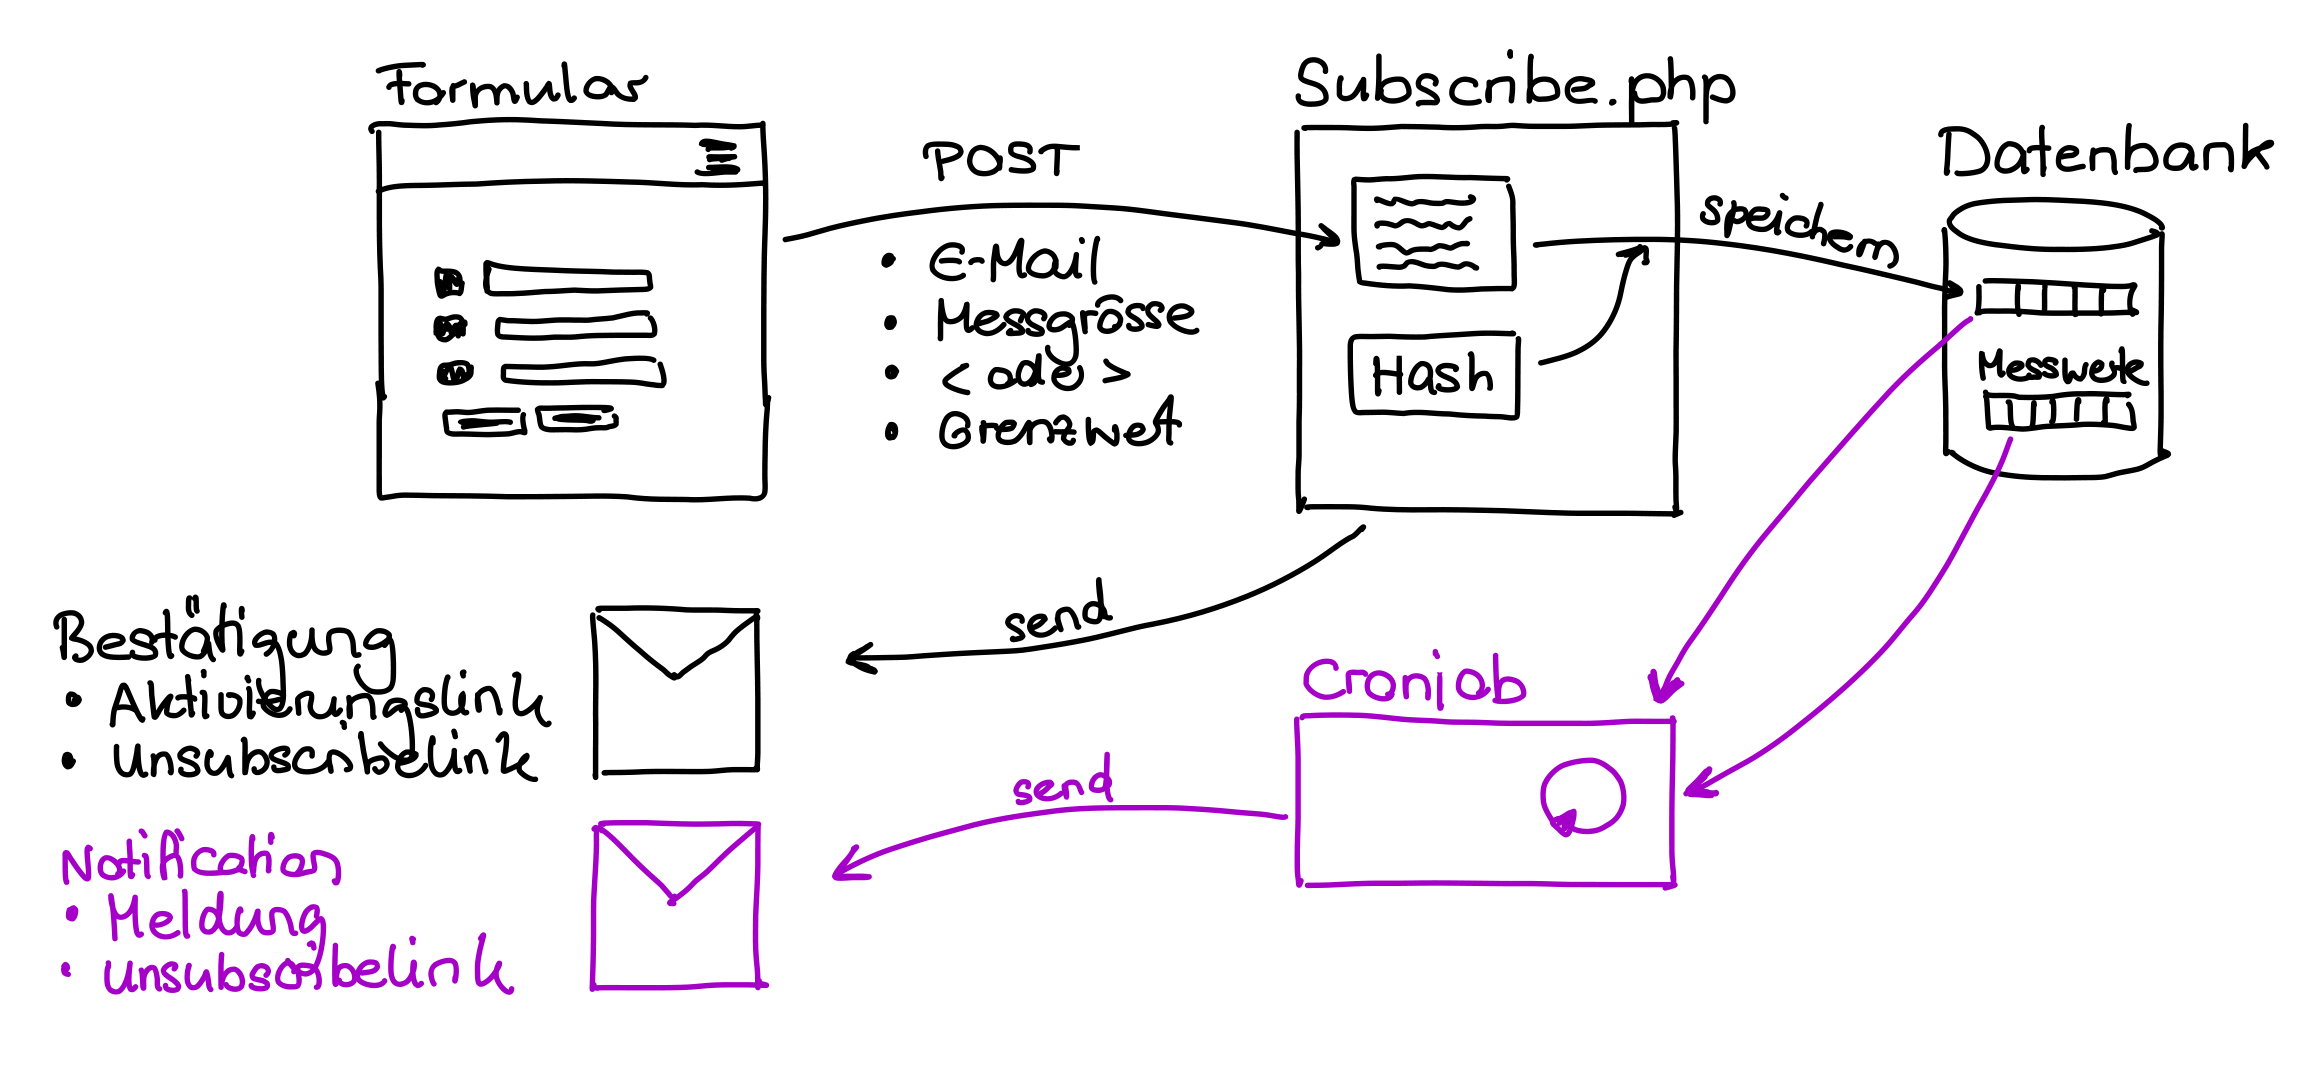
\includegraphics[width=\textwidth-2\fboxsep-2\fboxrule]{img/notificationKonzept}}
	\centering
	\caption{Funktionsprinzip des Benachrichtungsservices}
	\label{img:notificationKonzept}
\end{figure}

Der Benachrichtungsservice selbst basiert auf einem Cronjob, der einmal pro Stunde läuft. Das Prinzip ist in Abbildung \ref{img:notificationKonzept} in violett dargestellt. Der Cronjob ruft sämtliche Einträge in der Notification-Tabell ab und vergleicht sie mit den Messwerten. Sobald eine Bedingung erfüllt ist, wir ein Notification-Mail an die hinterlegete E-Mail-Adresse gesendet. Neben der eigentlichen Meldung ist ein Unsubscribelink vorhanden, damit der Benutzer den Benachritigungsservice abbestellen kann.

%% ############################################################################
%% Unterkapitel
%% ############################################################################
\subsection{Formular mit integrierter Überprüfung der Eingabe}
Das Formular des Benachrichtungsservices besteht aus vier Eingabe- bzw. Auswahlfeldern, wie in Abbildung \ref{img:notificationFE}, links, dargestellt. Zuoberst kann die gewünschte Messgrösse ausgewählt werden. Das Dropdown-Menü stellt sicher, dass nur Werte ausgewählt werden können, die von der Wetterstation zur Verfügung gestellt werden. Mit den Radio-Buttons kann ausgewält werden ob der Messwert grösser oder kleiner als der Grenzwert sein soll. Der Grenzwert wird als Zahl eingeben auf eine Stelle nach dem Komma genau. Zuletzt muss die E-Mail-Adresse, an welche die Benachrichtigung gesendet werden soll eingetragen werden. Durch Anklicken des Abonnieren-Buttons wird das Formular abgesendet.

\begin{figure}[h!]
  \fbox{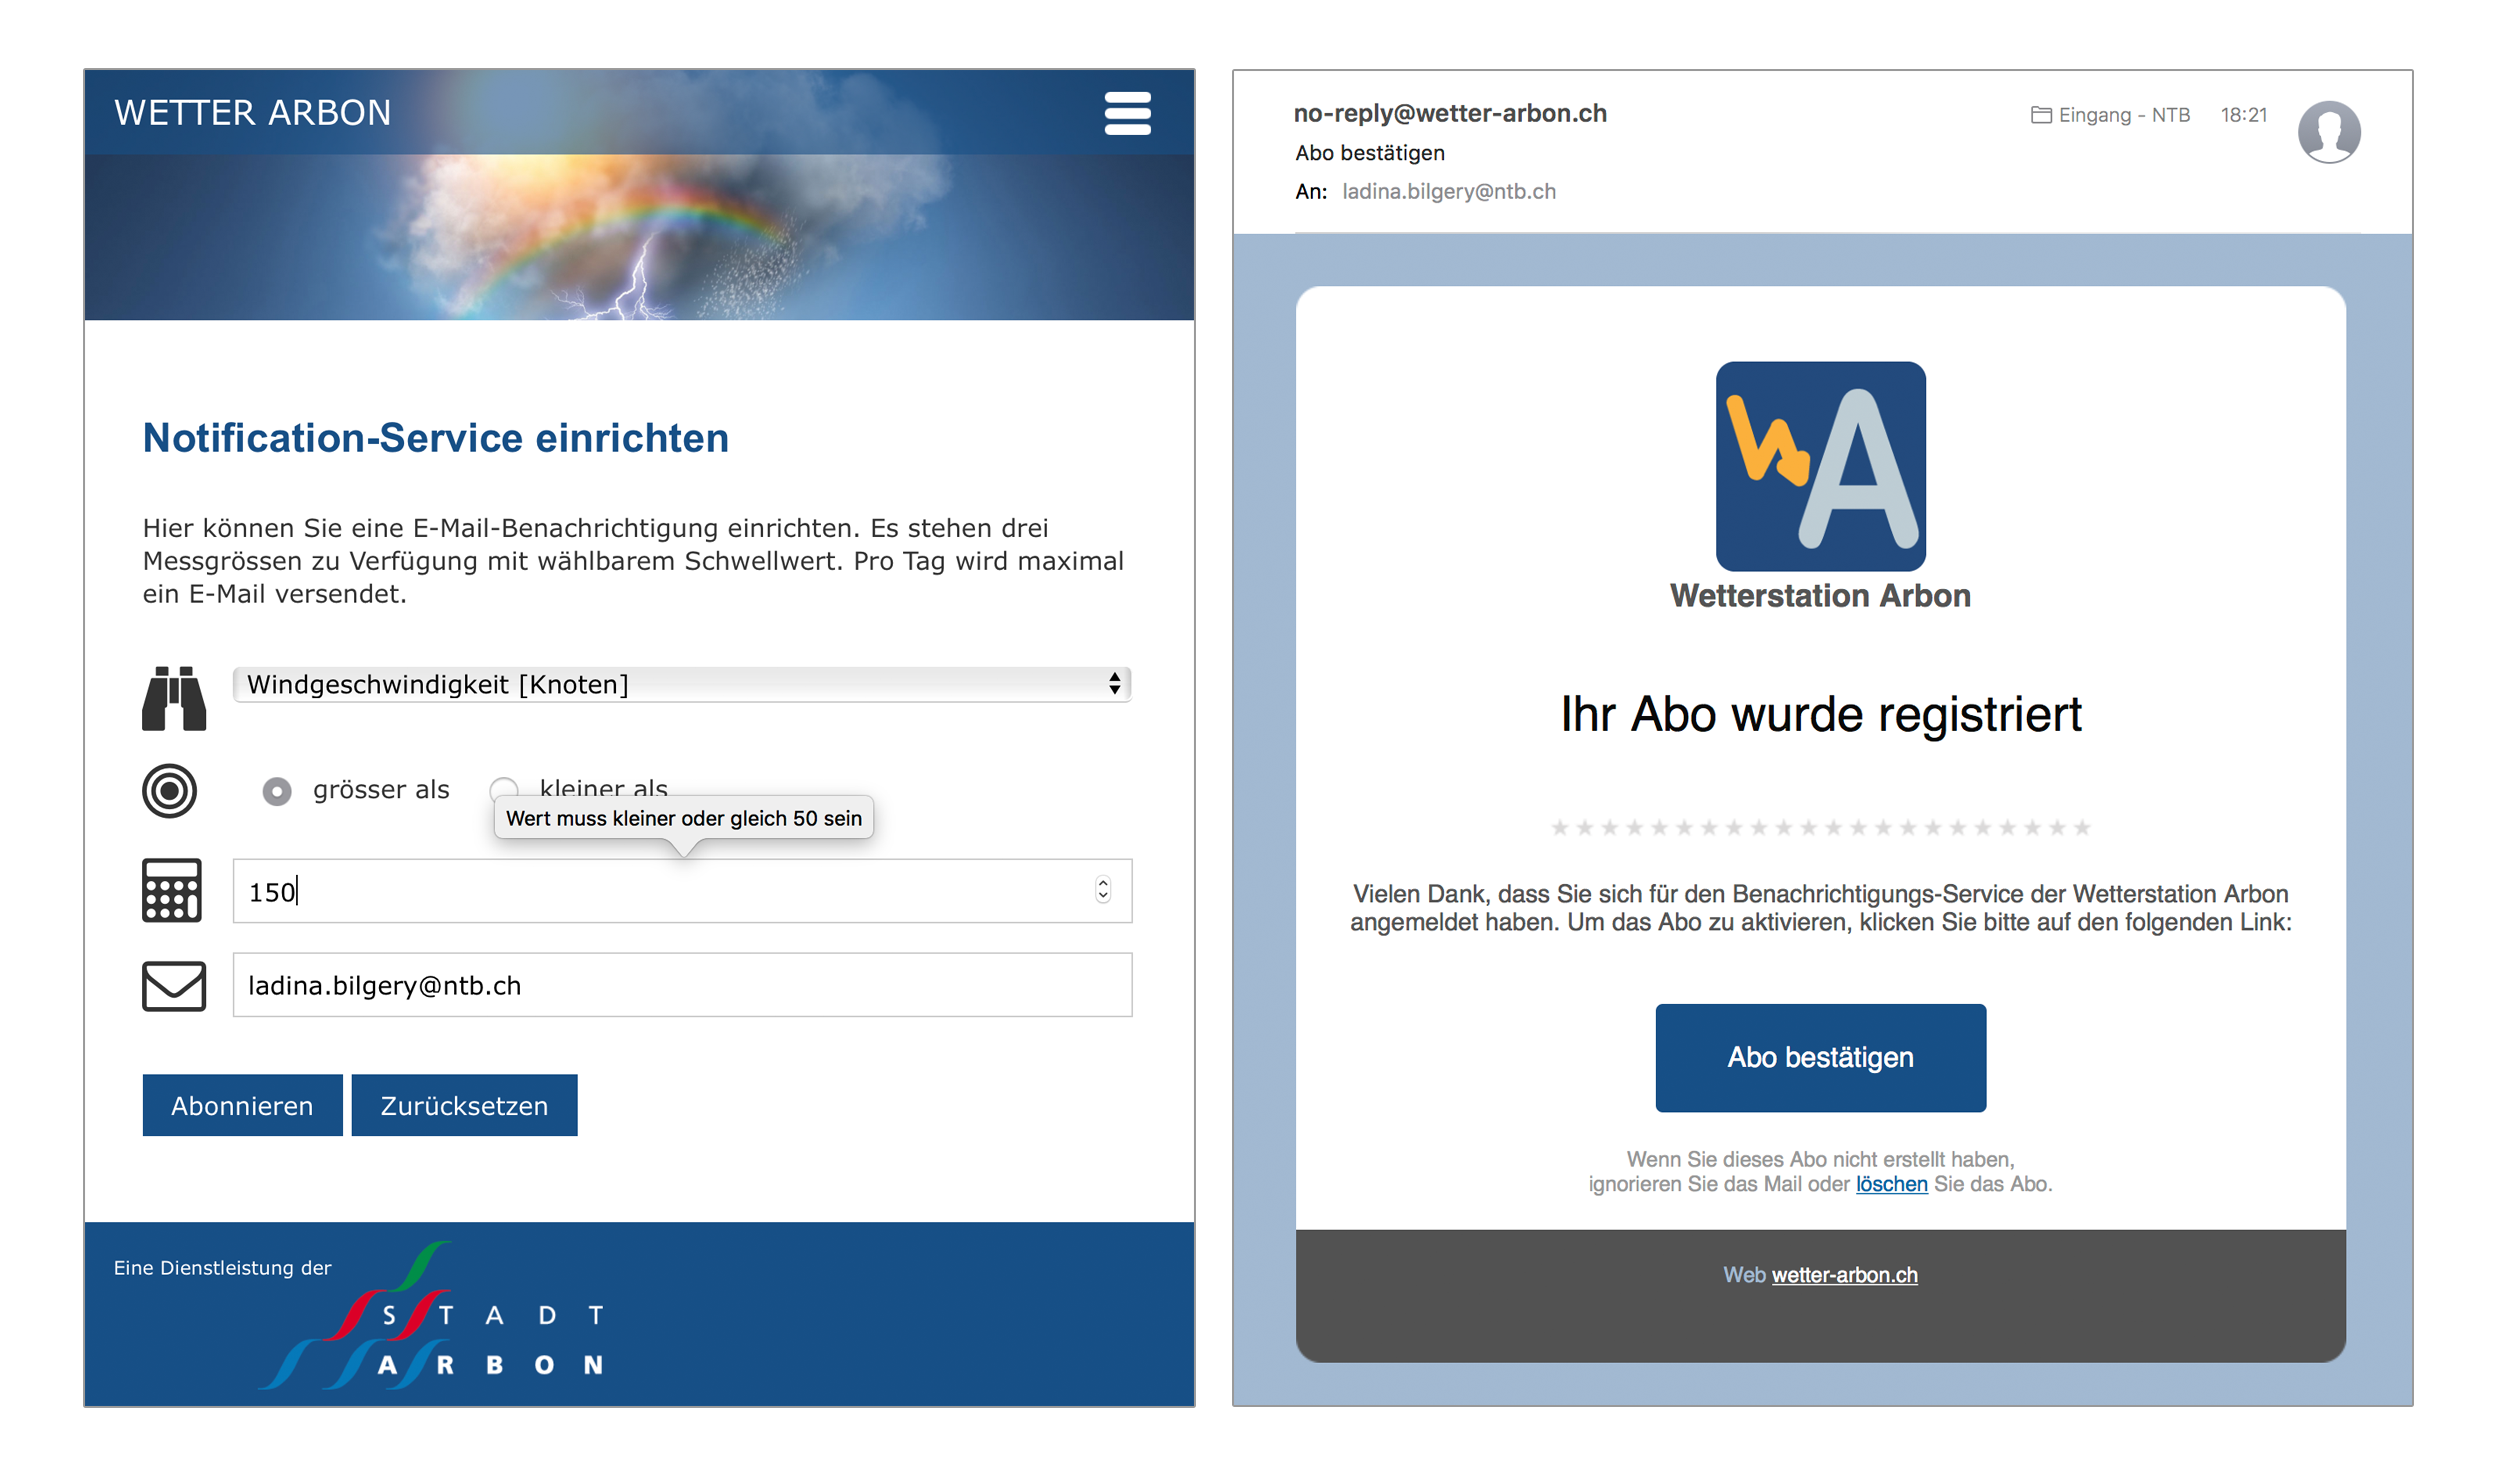
\includegraphics[width=\textwidth-2\fboxsep-2\fboxrule]{img/notificationFE}}
	\centering
	\caption{Eingabeformular mit Fehlerüberprüfung (rechts)}
	\label{img:notificationFE}
\end{figure}

Bisher musst die clientseitige Formularüberprüfung manuell programmierte werden bzw. eine JavaScript-Bibliothek verwendet werden. Unter HTML5 ist die Formularüberprüfung direkt integriert. Über die Defintion des \textit{type} und gegebenenfalls einiger Zusatzangaben, wird die  Überprüfung automtisch beim Absenden des Formulars durchgeführt und bei Fehlern direkt eine Meldung angezeigt. Der Wertebereich auf unsere Webseite ist zum Beispiel eingeschränkt auf Zahlen von 1 bis 50, wie in Listing \ref{lst:HTML5form} aufgezeigt. Wir nun ein Wert ausserhalb dieses Bereichs eingegeben, so erhält der Benutzer eine Fehlermeldung wie in Abbildung \ref{img:notificationFE}, rechts dargestellt und das Formular wird nicht abgesendet.

% Überprüfung der Eingaben
\begin{lstlisting}[label=lst:HTML5form,caption=Integrierte Formularüberprüfung mit HTML5, language=HTML5, style=htmlcssjs]
<!-- Auswahlmenue -->
<select name="measurand" required>
  <option value="" disabled selected>Messgrösse auswählen</option>
  <option value="windspeed">Windgeschwindigkeit</option>
</select>

<!-- Radio Button -->
<input type="radio" value="greater" checked>

<!-- Zahlenbereich -->
<input type="number" min="1" step="0.1" max="50" value="6">

<!-- E-Mail Adresse -->
<input type="email" placeholder="max.mustermann@web.ch" required>
\end{lstlisting}



%% ############################################################################
%% Unterkapitel
%% ############################################################################
\subsection{Identifikation des Abos via URL}
Die Tabelle für die Speicherung der Abos in der Datenbank enthält neben den vom Benutzer eingegbenen Daten noch weitere Einträge. Dies ist einerseits der Status des Abos d.h. aktiv oder inaktiv, den Zeitstempel des letzen Mails, sodass maximal einmal pro Tag ein Mail versendet wird, sowie den eindeutigen, nicht erratbaren Schlüssel (Hash), welcher für sämtliche Datenbank-Operationen benötigt wird.

% Bilder der DB-Tabellenstruktur?

Neben der \textit{subscribe.php}-Seite gibt es noch eine \textit{verify.php}-Seite und eine \textit{unsubscribe.php}-Seite. Diese führen jeweils die gewünschten Änderungen in der Datenbank aus. Zur Identifizierung des Abos enthält der Link sowohl die E-Mail-Adresse, als auch den Schlüssel (Hash) des entsprechenden Abos. Der Link für die Aktivierung des Abos lautet beispielhaft wie in Listing \ref{lst:verify} aufgeführt.

\begin{lstlisting}[label=lst:verify,caption=Beispiellink für die Aktivierung eines Abos, language=Python, style=py]
https://dev.wetter-arbon.ch/application/php/verify.php?
email=ladina.bilgery@ntb.ch&
hash=81f27f8a7d8766c72c0307a31327c1fad9007c6c3d33724ad2a5c0a8fe0df33d
\end{lstlisting}

Auf diese Weise kann auf Grund der aufgerufen Seite (subscribe, verify, unsubscribe) und dem Paar E-Mail und Schlüssel die Datenbankoperation genau definiert werden.
